% !TeX program = pdflatex
% !BIB program = biber
% !TeX TXS-program:compile = txs:///pdflatex
\documentclass[12pt,oneside]{report}

\usepackage[a4paper,margin=1in]{geometry}
\usepackage[T1]{fontenc}
\usepackage[utf8]{inputenc}
\usepackage[english]{babel}
\usepackage{mathptmx}
\usepackage{microtype}
\usepackage{setspace}
\usepackage{csquotes}
\usepackage{booktabs}
\usepackage{longtable}
\usepackage{tabularx}
\usepackage{array}
\usepackage{enumitem}
\usepackage{graphicx}
\usepackage{float}
\usepackage{caption}
\usepackage{xcolor}
\usepackage{tikz}
\usetikzlibrary{arrows.meta,positioning,shapes.geometric}
\usepackage{fancyhdr}
\usepackage{hyperref}
\usepackage{bookmark}
\usepackage[
  backend=biber,
  style=apa,
  sorting=nyt,
  sortcites=true,
  maxcitenames=2,
  maxbibnames=20,
  doi=true,
  url=true
]{biblatex}
\DeclareLanguageMapping{english}{english-apa}
\addbibresource{references.bib}

% -----------------------------------------------------------------------------
% EDIT THESE FIELDS IN TEXSTUDIO
% -----------------------------------------------------------------------------
\newcommand{\ResearchTitle}{Sari-SaaS: Design and Development of a Secure, Offline-Capable Unified Commerce Management Platform for Philippine MSMEs}
\newcommand{\ResearchAuthor}{[Researcher Name]}
\newcommand{\Institution}{[Institution Name]}
\newcommand{\DepartmentName}{[College or Department]}
\newcommand{\DegreeProgram}{[Degree Program]}
\newcommand{\ResearchAdviser}{[Research Adviser]}
\newcommand{\SubmissionDate}{August 2026}

\hypersetup{
  colorlinks=true,
  linkcolor=black,
  citecolor=black,
  urlcolor=blue,
  pdftitle={\ResearchTitle},
  pdfauthor={\ResearchAuthor}
}

\setlength{\parindent}{0.5in}
\setlength{\parskip}{0pt}
\setlength{\emergencystretch}{3em}
\setlength{\headheight}{14pt}
\doublespacing
\captionsetup{font=small,labelfont=bf}
\setlist{nosep,leftmargin=0.35in}
\renewcommand{\arraystretch}{1.25}
\newcolumntype{Y}{>{\raggedright\arraybackslash}X}
\newcolumntype{L}[1]{>{\raggedright\arraybackslash}p{#1}}

\pagestyle{fancy}
\fancyhf{}
\fancyhead[R]{\small Sari-SaaS Research and Development Manuscript}
\fancyfoot[C]{\thepage}
\renewcommand{\headrulewidth}{0.4pt}

\begin{document}

\hypersetup{pageanchor=false}
\begin{titlepage}
  \centering
  \vspace*{0.8in}
  {\Large\bfseries \ResearchTitle\par}
  \vspace{1.2in}
  {\large A Developmental Research Manuscript\par}
  \vspace{0.35in}
  {\large Presented to\par}
  {\large \DepartmentName\par}
  {\large \Institution\par}
  \vspace{0.9in}
  {\large In Partial Fulfillment of the Requirements for\par}
  {\large \DegreeProgram\par}
  \vfill
  {\large \ResearchAuthor\par}
  \vspace{0.25in}
  {\large Adviser: \ResearchAdviser\par}
  \vspace{0.5in}
  {\large \SubmissionDate\par}
\end{titlepage}
\hypersetup{pageanchor=true}

\pagenumbering{roman}

\chapter*{Document Status}
\addcontentsline{toc}{chapter}{Document Status}
This manuscript documents an active software research and development project.
It reports verified characteristics of the current Sari-SaaS prototype and
presents a formal protocol for the field evaluation that should follow. It does
not claim that merchant surveys, comparative task experiments, or statistical
tests have already been completed. Sections describing future participants,
instruments, acceptance thresholds, or hypotheses are therefore written as a
proposed evaluation plan. This distinction is necessary to preserve research
integrity and prevent technical verification results from being misrepresented
as human-subject findings.

\chapter*{Abstract}
\addcontentsline{toc}{chapter}{Abstract}
Micro, small, and medium enterprises (MSMEs) account for 99.63\% of registered
business establishments in the Philippines, yet many microentrepreneurs still
manage online orders, payment evidence, stock, and delivery coordination across
separate applications and manual records. This developmental study designs and
implements Sari-SaaS, a mobile-first commerce management platform for fragmented
merchant workflows, intermittent connectivity, and resource-constrained
devices. It applies design science research with Scrum-based iterative
development. The TypeScript artifact combines web, mobile, application
programming interface, shared-domain, and Supabase PostgreSQL components.
Security controls include tenant-scoped row-level security, encrypted integration
credentials, short-lived single-use authorization state, signed webhook
verification, inactivity-based sign-out, and server-only integration writes.
The prototype implements email magic-link authentication, merchant onboarding,
an English/Tagalog dashboard, order and inventory views, and secure connection
foundations for Facebook, Instagram, TikTok Shop, WooCommerce, and Shopify.
Repository linting, static type checking, provider-security tests, database
migration, and production builds completed successfully. Full offline mutation
synchronization, payment OCR, logistics booking, and transformation of provider
events into local orders remain incomplete. A field evaluation with Philippine
MSME merchants is therefore proposed using task completion, error rates, the
System Usability Scale, Technology Acceptance Model constructs, and ISO/IEC
25010 quality criteria. The principal contribution is a context-sensitive,
security-oriented design that translates fragmented social-commerce operations
into a testable artifact without overstating prototype maturity.

\noindent\textbf{Keywords:} Philippine MSMEs, social commerce, offline-capable
systems

\tableofcontents
\listoftables
\listoffigures
\clearpage
\pagenumbering{arabic}

\chapter{Introduction}

\section{Background of the Study}
MSMEs form the numerical foundation of the Philippine business sector. The
Department of Trade and Industry reported that 1,236,908 of 1,241,476 registered
establishments in 2024 were MSMEs, equivalent to 99.63\% of all establishments
\parencite{dti2024msme}. Their scale makes improvements in MSME operations
relevant not only to individual firms but also to employment, local supply
chains, and inclusive economic participation. The Asian Development Bank (ADB)
similarly treats MSMEs as a central driver of resilient and inclusive growth
across Asia and the Pacific \parencite{adb2024monitor}.

Commercial activity is also becoming increasingly digital. Digital retail
payments represented 57.4\% of transaction volume and 59.0\% of transaction
value in the Philippines in 2024 \parencite{bsp2024payments}. For small
merchants, however, digitalization does not necessarily produce a coherent
operating process. A seller may receive inquiries through Facebook or
Instagram, accept payment through a mobile wallet, encode the order in a
notebook or spreadsheet, update stock separately, and open another application
to arrange delivery. Philippine microentrepreneurs interviewed by
\textcite{romero2023women} commonly used Facebook for selling and reported
benefits from e-commerce, but they also experienced technical problems, slow
connectivity, competition, and fraudulent or difficult customer interactions.

This fragmented setting creates an information-management problem. Separate
records increase repeated encoding, delayed responses, missed orders, inventory
errors, and weak transaction traceability. The Internet Transactions Act of
2023 also places greater emphasis on trust, merchant accountability, consumer
protection, secure internet transactions, and data privacy
\parencite{philippines2023ita}. A useful MSME platform must therefore do more
than provide a polished dashboard: it must coordinate existing channels,
preserve records, protect personal and commercial data, and remain dependable
when connectivity is poor.

Sari-SaaS was conceived as a unified commerce command platform for Philippine
MSMEs. The project prioritizes low-cost Android devices, text-first interaction,
English and Tagalog localization, offline-capable workflows, and integration
with the services merchants already use \parencite{sariSpec2026}. Instead of
requiring sellers to abandon social networks, wallets, and courier platforms,
the system provides a common operational layer for orders, inventory, payments,
messages, and delivery activities.

\section{Statement of the Problem}
Philippine MSME merchants who sell through multiple digital channels may lack a
single, secure, and connectivity-resilient system for managing the complete
transaction lifecycle. The project addresses five related problems:

\begin{enumerate}
  \item Order information is distributed across social networks, online-store
  platforms, notes, and spreadsheets.
  \item Payment verification and reconciliation often depend on manual review
  and repeated encoding.
  \item Inventory records can become inconsistent when sales are recorded late
  or separately from stock updates.
  \item Courier booking and customer updates require switching between systems.
  \item Existing digital workflows may not provide appropriate tenant
  isolation, auditability, privacy safeguards, accessibility, or graceful
  operation during unstable connectivity.
\end{enumerate}

The central research problem is therefore how to design, implement, and evaluate
a unified commerce management artifact that responds to these operational and
technical conditions without introducing unacceptable security or usability
burdens.

\section{Research Questions}
This study is guided by the following questions:

\begin{enumerate}
  \item How can a mobile-first system consolidate order, inventory, payment,
  channel, and logistics workflows used by Philippine MSMEs?
  \item How can the platform remain responsive and preserve merchant actions
  during intermittent or unavailable network connectivity?
  \item What controls are necessary to protect merchant data, integration
  credentials, authorization callbacks, and webhook events in a multi-tenant
  software-as-a-service environment?
  \item To what extent does the implemented artifact satisfy selected
  ISO/IEC 25010 quality characteristics, particularly functional suitability,
  performance efficiency, compatibility, interaction capability, reliability,
  security, maintainability, and flexibility?
  \item In a future field evaluation, how usable, useful, and easy to learn is
  Sari-SaaS for Philippine MSME owners and operators compared with their current
  fragmented workflow?
\end{enumerate}

\section{Objectives of the Study}
\subsection{General Objective}
The general objective is to design, develop, and evaluate a secure,
offline-capable, and localized unified commerce management platform for
Philippine MSMEs.

\subsection{Specific Objectives}
The study specifically aims to:

\begin{enumerate}
  \item model a unified transaction workflow for orders, payments, inventory,
  sales channels, and delivery;
  \item implement a shared web, mobile, API, and database architecture with
  reusable domain types and validation rules;
  \item provide immediate local interaction and a recoverable synchronization
  design for unstable connectivity;
  \item implement tenant isolation, credential encryption, replay-resistant
  authorization state, signed webhook verification, and secure session
  handling;
  \item support English and Tagalog interfaces with accessible navigation and
  touch targets;
  \item verify the prototype through migration checks, static analysis,
  automated tests, and production builds; and
  \item define a reproducible merchant-centered evaluation protocol for
  usability, acceptance, task efficiency, reliability, and software quality.
\end{enumerate}

\section{Significance of the Study}
\textbf{MSME owners and staff.} The system may reduce repeated encoding,
application switching, missed follow-ups, and uncertainty about stock or payment
status. Its localization and low-bandwidth design seek to lower the effort
needed to adopt structured digital operations.

\textbf{Customers.} Better transaction records and timely status updates may
improve transparency, order accuracy, and access to transaction evidence.

\textbf{Government and MSME support institutions.} The artifact offers a
technical reference for programs that promote e-commerce participation,
traceability, digital payments, and responsible digitalization.

\textbf{Software developers and researchers.} The project provides an applied
case of design science, local-first principles, multi-tenant security, and
third-party commerce integration under emerging-market constraints.

\textbf{Future researchers.} The proposed instruments, acceptance thresholds,
and traceability matrix can support replication, comparative evaluation, and
longitudinal study after deployment.

\section{Scope and Delimitations}
The research artifact includes a Next.js web application, an Expo mobile
application scaffold, a Fastify API, shared TypeScript domain packages, and a
Supabase PostgreSQL database. The functional scope covers authentication and
merchant onboarding, dashboard indicators, order and inventory views, channel
connection metadata, and a secure webhook intake queue. The channel framework
supports Facebook, Instagram, TikTok Shop, WooCommerce, and Shopify at different
levels of provider readiness.

The study does not claim that all provider approvals, payment gateways, OCR
models, logistics APIs, offline synchronization rules, and production
observability workflows are complete. Provider webhook events are accepted and
deduplicated, but automatic transformation of all events into local orders and
stock movements remains future work. The manuscript also does not report field
survey outcomes, financial impact, or legal compliance certification. Legal and
standards references inform design requirements but do not replace professional
legal, privacy, accounting, or security review.

\section{Definition of Terms}
\begin{description}[style=nextline,leftmargin=0.3in]
  \item[Design science research.] A research paradigm in which a purposeful
  artifact is created and evaluated to address a relevant organizational
  problem.
  \item[Local-first or offline-capable.] A design approach in which useful work
  can continue locally and synchronize when communication becomes available
  \parencite{kleppmann2019localfirst}.
  \item[MSME.] A micro, small, or medium enterprise as classified by Philippine
  policy or statistical authorities.
  \item[OAuth.] A delegated authorization framework through which a user grants
  an application limited access without sharing the user's platform password.
  \item[Progressive web application (PWA).] A web application enhanced with
  installability and platform capabilities while retaining browser delivery.
  \item[Row-level security (RLS).] Database policy enforcement that limits
  accessible rows according to the authenticated user and store relationship.
  \item[Webhook.] A provider-initiated HTTPS request that communicates an event
  to another system.
\end{description}

\chapter{Review of Related Literature and Systems}

\section{MSMEs and Digitalization in the Philippine Context}
The dominance of MSMEs in the Philippine establishment count establishes the
relevance of tools designed for small operating teams rather than enterprise
departments \parencite{dti2024msme}. The ADB's regional monitoring emphasizes
that resilient MSME ecosystems require more than access to technology; they
also depend on finance, skills, supportive institutions, market access, and
appropriate policy \parencite{adb2024monitor}. This broader view cautions
against treating software alone as a complete intervention.

Philippine evidence shows that microentrepreneurs adopt e-commerce pragmatically.
\textcite{romero2023women} described bricolage behavior among women
microentrepreneurs: available tools and resources were combined to sustain
online participation. Such behavior supports an integration-oriented system
strategy. A platform is more likely to fit existing practice when it coordinates
familiar channels rather than requiring immediate migration to an unfamiliar
and comprehensive enterprise system.

At the same time, digitalization can create new burdens if technology is costly,
complex, unreliable, or poorly aligned with operating conditions. The research
problem is therefore not simply whether merchants use digital platforms, but
whether their combined workflow is understandable, efficient, secure, and
recoverable.

\section{Social Commerce and Fragmented Operations}
Social commerce combines social interaction with commercial discovery,
negotiation, and transaction activity. For microenterprises, social networks
lower the cost of market access, but they also mix customer communication with
order capture. Conversations, comments, screenshots, and order details may not
produce structured records automatically. This creates a need for a unifying
layer that can identify the channel while normalizing orders and customer
activity into shared domain objects.

The current Sari-SaaS design treats Facebook, Instagram, TikTok Shop,
WooCommerce, and Shopify as external systems. It uses delegated authorization
or store-generated credentials rather than collecting platform passwords. This
approach is consistent with OAuth security guidance that discourages password
credential grants and favors authorization-code flows, constrained scopes,
redirect validation, and replay protection \parencite{rfc9700oauth}.

\section{Digital Payments and Reconciliation}
The expansion of digital payments establishes both an opportunity and a record
management burden. BSP measurements show that a majority of Philippine retail
payment volume is now digital \parencite{bsp2024payments}. A merchant may still
need to match payment evidence to a particular order, detect duplicate
references, and preserve a traceable state change. The Sari-SaaS specification
therefore proposes two paths: signed gateway webhooks when a direct integration
exists and on-device optical character recognition (OCR) for payment
screenshots.

Client-side OCR can reduce transmission of payment screenshots, although its
accuracy and resource cost must be measured on target devices. Tesseract's
lineage as an adaptable OCR engine is well documented \parencite{smith2007ocr},
but a general OCR engine does not by itself establish acceptable accuracy for
GCash or Maya screenshots. A domain-specific test set, confidence thresholds,
manual fallback, and false-match analysis remain necessary.

\section{Offline-Capable and Local-First Design}
Local-first research argues that a local copy can support immediate access and
work during disconnection while synchronization restores collaboration later
\parencite{kleppmann2019localfirst}. These principles are relevant to merchants
who use prepaid data or encounter unstable mobile signals. A local-first design
can reduce blocking network round trips, but it also introduces conflict,
ordering, durability, and reconciliation problems.

The project currently proposes IndexedDB for web storage, SQLite for mobile
storage, and a mutation queue that synchronizes deltas. Last-write-wins may be
acceptable for low-risk profile fields but is insufficient for all inventory
and payment conflicts. Stock quantities, payment state, and fulfillment events
require domain-specific idempotency keys, monotonic state transitions, and
auditable conflict handling. The literature therefore supports offline work as
a design goal while also demonstrating why synchronization must be evaluated as
a subsystem rather than treated as a browser caching feature.

\section{Technology Acceptance and Information-System Success}
The Technology Acceptance Model identifies perceived usefulness and perceived
ease of use as determinants of user acceptance \parencite{davis1989tam}. This
model is appropriate to the target population because Sari-SaaS competes with
simple but familiar practices such as notebooks and direct use of social media.
An artifact can be technically sophisticated and still fail if merchants do not
believe it saves time or if initial setup appears difficult.

The DeLone and McLean model connects system quality, information quality,
service quality, use, satisfaction, and net benefits
\parencite{delone2003success}. Together, these frameworks justify evaluating
more than interface preference. The proposed study measures task success and
errors, perceived usefulness and ease, satisfaction, reliability, and the
quality of operational information.

\section{Software Quality, Accessibility, and Security}
ISO/IEC 25010:2023 defines a product quality model with nine characteristics
that can guide requirements and evaluation throughout the software lifecycle
\parencite{iso25010}. Sari-SaaS prioritizes functional suitability,
performance efficiency, compatibility, interaction capability, reliability,
security, maintainability, and flexibility. Safety is considered where
incorrect status or inventory information could influence merchant decisions.

WCAG 2.2 organizes accessibility around perceivable, operable, understandable,
and robust content and provides testable success criteria for web interfaces
\parencite{w3c2024wcag}. The project's text-first controls, visible labels,
responsive layout, high contrast, and large touch targets are consistent with
that direction, but formal conformance must still be audited across complete
pages and interaction states.

Security is treated as an architectural quality rather than a final checklist.
The Data Privacy Act regulates the processing lifecycle of personal data and
establishes accountability obligations \parencite{philippines2012dpa}. OWASP
ASVS provides verifiable web-application security requirements
\parencite{owasp2025asvs}, while NIST digital identity guidance informs
authentication and session controls \parencite{nist2025identity}. For external
channels, OAuth best current practice supports authorization-code exchange,
state validation, least privilege, TLS, and protection against token replay and
redirect attacks \parencite{rfc9700oauth}.

\section{Legal and Regulatory Context}
The Internet Transactions Act applies to covered business-to-business and
business-to-consumer transactions involving the Philippine market. It promotes
trust, consumer protection, secure transactions, data privacy, transparent
offers, and identifiable parties \parencite{philippines2023ita}. The law
supports the project's emphasis on merchant profiles, transaction records,
receipt-ready data, and traceability. Nevertheless, software features are not
equivalent to certification. Production deployment requires review of the Act's
implementing rules, consumer remedies, registration obligations, tax and
invoicing requirements, retention policies, and provider terms.

\section{Synthesis and Research Gap}
The literature supports digital commerce participation, offline-capable
interaction, usable systems, and security controls, but these concerns are often
studied or implemented separately. Philippine microentrepreneurs commonly
assemble multiple general-purpose tools, while enterprise commerce systems may
assume stable connectivity, dedicated staff, or formal online-store operations.
The research gap addressed by Sari-SaaS is the design and evaluation of a single
localized artifact that coordinates social channels, online stores, payment
evidence, stock, and delivery while explicitly accounting for low-resource
devices, connectivity interruptions, multi-tenant security, and merchant
acceptance.

\chapter{Methodology}

\section{Research Design}
The study uses design science research because its primary output is a purposeful
information-system artifact. \textcite{hevner2004designscience} describe design
science as the construction and evaluation of artifacts that extend human and
organizational capabilities. The process follows the six activities proposed by
\textcite{peffers2007dsrm}: problem identification and motivation, definition of
solution objectives, design and development, demonstration, evaluation, and
communication.

The study is also developmental and mixed-method in its proposed evaluation.
Technical verification produces quantitative measures such as build success,
latency, task completion, error counts, and synchronization outcomes. Merchant
testing adds scaled acceptance responses and qualitative observations or
interviews. No causal claim will be made without an appropriate comparative
design and sufficient data.

\begin{table}[H]
\centering
\caption{Mapping of Design Science Activities to the Sari-SaaS Study}
\label{tab:dsrm}
\begin{tabularx}{\textwidth}{L{0.25\textwidth}Y}
\toprule
\textbf{DSR activity} & \textbf{Application in this study} \\
\midrule
Problem identification & Analyze fragmented merchant workflows, connectivity
constraints, transaction traceability, and security risks. \\
Solution objectives & Define a localized, mobile-first, integrated, secure, and
offline-capable commerce platform. \\
Design and development & Build the monorepo, shared domain model, web/mobile
clients, API, database policies, and provider integration layer. \\
Demonstration & Execute representative onboarding, order, inventory, and channel
connection workflows in a controlled environment. \\
Evaluation & Perform technical verification and a future merchant-centered
usability and acceptance study. \\
Communication & Produce the software repository, architecture decisions,
technical guides, and this research manuscript. \\
\bottomrule
\end{tabularx}
\end{table}

\section{Development Method}
Development is organized using Scrum with a two-week sprint model and a
prioritized product backlog \parencite{sariScrum2026}. Scrum is an iterative
framework based on transparency, inspection, and adaptation
\parencite{schwaber2020scrum}. The backlog groups work into authentication,
offline data, messaging, payment reconciliation, orders, inventory, dashboard,
integrations, logistics, compliance, billing, and analytics.

Each increment should satisfy a definition of done that includes acceptance
criteria, automated checks, target-device review, security impact review, and
documentation. Features involving external providers are not considered
complete merely because a UI card exists; authorization, callback validation,
credential protection, webhook authenticity, error recovery, and event
processing must also be demonstrated.

\section{Conceptual Framework}
The conceptual framework combines an input-process-output structure with
acceptance and quality outcomes. Figure~\ref{fig:conceptual} shows how merchant
needs, technical constraints, regulatory duties, and design knowledge enter an
iterative design-science process. The output is the Sari-SaaS artifact, while
evaluation considers software quality, user acceptance, and operational effect.

\begin{figure}[H]
\centering
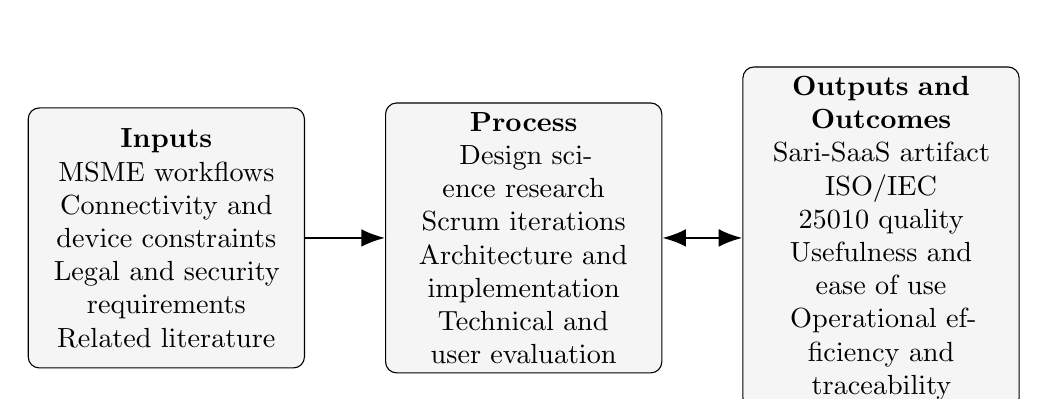
\begin{tikzpicture}[
  node distance=0.40in,
  box/.style={draw,rounded corners,align=center,text width=0.27\textwidth,
    minimum height=1.30in,fill=gray!8},
  arrow/.style={-{Latex[length=3mm]},thick}
]
\node[box] (input) {\textbf{Inputs}\\MSME workflows\\Connectivity and device
constraints\\Legal and security requirements\\Related literature};
\node[box,right=of input] (process) {\textbf{Process}\\Design science
research\\Scrum iterations\\Architecture and implementation\\Technical and
user evaluation};
\node[box,right=of process] (output) {\textbf{Outputs and Outcomes}\\Sari-SaaS
artifact\\ISO/IEC 25010 quality\\Usefulness and ease of use\\Operational
efficiency and traceability};
\draw[arrow] (input) -- (process);
\draw[thick,{Latex[length=3mm]}-{Latex[length=3mm]}] (process) -- (output);
\end{tikzpicture}
\caption{Conceptual framework of the study}
\label{fig:conceptual}
\end{figure}

\section{System Architecture}
The artifact uses a monorepo so web, mobile, API, database, and shared packages
can evolve under common type definitions. Figure~\ref{fig:architecture} presents
the logical architecture.

\begin{figure}[H]
\centering
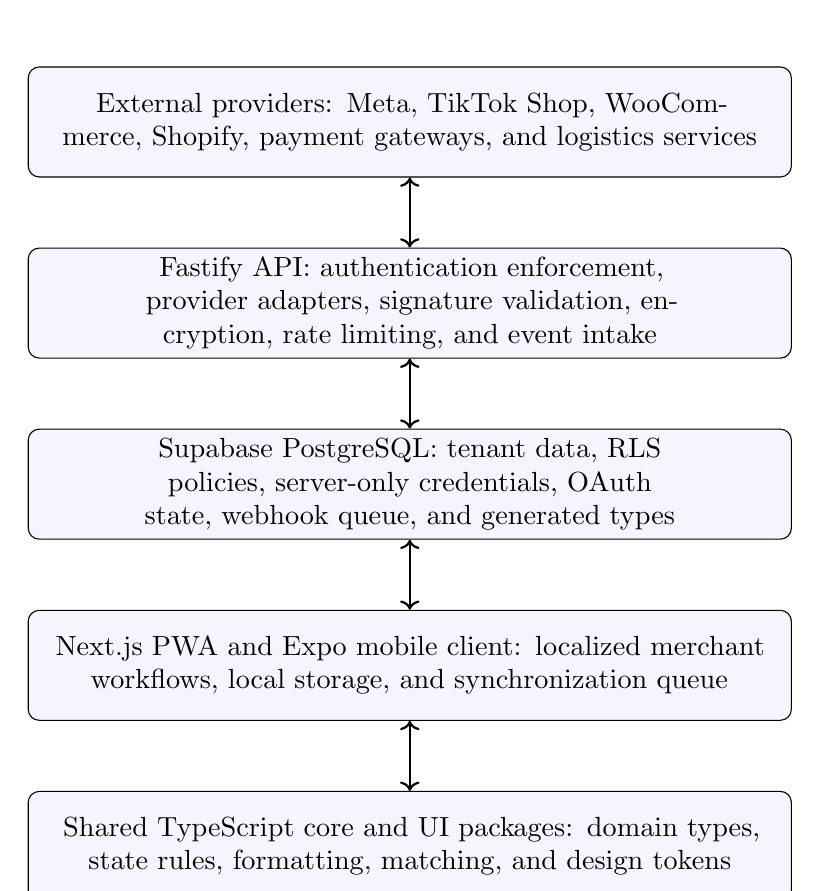
\begin{tikzpicture}[
  node distance=0.35in,
  layer/.style={draw,rounded corners,align=center,text width=0.78\textwidth,
    minimum height=0.55in,fill=blue!4},
  arrow/.style={-{Latex[length=2.5mm]},thick}
]
\node[layer] (channels) {External providers: Meta, TikTok Shop, WooCommerce,
Shopify, payment gateways, and logistics services};
\node[layer,below=of channels] (api) {Fastify API: authentication enforcement,
provider adapters, signature validation, encryption, rate limiting, and event
intake};
\node[layer,below=of api] (db) {Supabase PostgreSQL: tenant data, RLS policies,
server-only credentials, OAuth state, webhook queue, and generated types};
\node[layer,below=of db] (clients) {Next.js PWA and Expo mobile client: localized
merchant workflows, local storage, and synchronization queue};
\node[layer,below=of clients] (shared) {Shared TypeScript core and UI packages:
domain types, state rules, formatting, matching, and design tokens};
\draw[arrow,<->] (channels) -- (api);
\draw[arrow,<->] (api) -- (db);
\draw[arrow,<->] (db) -- (clients);
\draw[arrow,<->] (clients) -- (shared);
\end{tikzpicture}
\caption{Logical architecture of Sari-SaaS}
\label{fig:architecture}
\end{figure}

\section{Data and Security Design}
The primary entities are users, stores, orders, payments, messages, inventory,
shipments, integration metadata, encrypted integration credentials, webhook
events, and synchronization records. Store ownership forms the tenant boundary.
Browser clients may read or modify only rows allowed by RLS policies, while
credential and authorization tables are restricted to the server service role.

The security design applies the following controls:

\begin{enumerate}
  \item short-lived email sign-in links and inactivity-based session timeout;
  \item per-store authorization and database RLS;
  \item AES-256-GCM encryption for third-party credentials with contextual
  authenticated data;
  \item hashed, short-lived, single-use authorization state;
  \item server-side token exchange and absence of provider secrets in browser
  environment variables;
  \item provider-specific HMAC verification over the unchanged webhook body;
  \item deduplication by provider and external event identifier;
  \item HTTPS requirements, strict Shopify domain validation, and public-address
  validation with DNS pinning for merchant-supplied WooCommerce hosts;
  \item API rate limiting and redaction of authorization-bearing request data;
  and
  \item automatic credential removal from local storage when an integration is
  disconnected or a Shopify uninstall event is received.
\end{enumerate}

These controls are informed by ASVS and OAuth guidance but require independent
penetration testing before production assurance can be claimed
\parencite{owasp2025asvs,rfc9700oauth}.

\section{Development and Evaluation Environment}
The reference environment uses Node.js 20 or later, pnpm workspaces,
TypeScript, Next.js, Expo, Fastify, and Supabase PostgreSQL. The repository
defines lint, type-check, test, build, migration, and type-generation commands.
Testing should cover a desktop browser, a low-cost Android device with 3 GB of
memory, and network profiles representing stable broadband, weak mobile data,
intermittent connection, and complete disconnection.

\section{Proposed Participants and Sampling}
The field evaluation should recruit Philippine MSME owners or staff who directly
perform at least two of the following: receive online orders, confirm digital
payments, update inventory, communicate with customers, or arrange delivery.
Purposive sampling is appropriate for initial formative evaluation because the
artifact targets a specific operational role. A proposed initial sample is 30
to 50 participants across micro and small enterprises, with diversity in age,
device capability, location, language preference, and primary sales channel.

The final sample size should be confirmed through the institution's research
protocol and the intended statistical analysis. A small formative usability
round may precede the larger evaluation to identify severe interface defects.
Participants must provide informed consent, and no provider password, live
payment credential, or unnecessary customer data should be collected.

\section{Proposed Instruments and Measures}
\begin{longtable}{L{0.24\textwidth}L{0.32\textwidth}L{0.35\textwidth}}
\caption{Proposed Evaluation Measures}\label{tab:measures}\\
\toprule
\textbf{Construct} & \textbf{Measure} & \textbf{Purpose} \\
\midrule
\endfirsthead
\toprule
\textbf{Construct} & \textbf{Measure} & \textbf{Purpose} \\
\midrule
\endhead
Task effectiveness & Completion, assistance, critical errors, and data accuracy
& Determine whether merchants can complete core workflows correctly. \\
Task efficiency & Completion time, taps/clicks, repeated encoding, and app
switches & Compare operational effort with the current workflow. \\
Usability & Ten-item System Usability Scale (SUS) & Produce a standardized
summary usability score \parencite{brooke1996sus,bangor2008sus}. \\
Acceptance & Perceived usefulness, perceived ease of use, and behavioral
intention items & Evaluate adoption-related perceptions based on TAM
\parencite{davis1989tam}. \\
Software quality & Expert rubric derived from ISO/IEC 25010 & Assess product
quality characteristics and documented evidence \parencite{iso25010}. \\
Accessibility & WCAG 2.2 automated and manual checks & Examine keyboard access,
labels, contrast, reflow, focus, and target sizing \parencite{w3c2024wcag}. \\
Reliability & Offline writes, reconnect synchronization, duplicate events,
retries, and recovery & Measure continuity and integrity under network change. \\
Security & Authorization, RLS, tenant isolation, secret exposure, signature,
replay, and SSRF test cases & Verify selected controls against documented
requirements \parencite{owasp2025asvs}. \\
\bottomrule
\end{longtable}

\section{Proposed Test Tasks}
Participants should complete representative tasks using synthetic data:

\begin{enumerate}
  \item sign in, complete store onboarding, and switch the interface language;
  \item record a walk-in or direct sale and review its payment state;
  \item add or inspect inventory and identify a low-stock product;
  \item locate pending payments and return to the dashboard;
  \item connect a sandbox or development sales channel where provider access is
  available;
  \item continue a supported action during simulated disconnection and verify
  its state after reconnection; and
  \item sign out or allow the inactivity timeout to protect the session.
\end{enumerate}

No task should use a participant's production credentials or real customer
records. Provider connection testing should use development shops, test users,
and revocable credentials.

\section{Data Analysis Plan}
Descriptive statistics should summarize task completion, error rates, times,
SUS scores, quality ratings, and acceptance constructs. Internal consistency of
multi-item scales should be assessed before computing composite scores. If the
same participants perform a baseline workflow and the Sari-SaaS workflow,
paired analysis may be used after checking distributional assumptions.
Qualitative observations should be coded into recurring themes such as
navigation, terminology, trust, connectivity, setup burden, and perceived
usefulness.

The following hypotheses may be tested after sufficient field data exist:

\begin{description}[leftmargin=0.45in]
  \item[H1.] Perceived ease of use is positively associated with behavioral
  intention to use Sari-SaaS.
  \item[H2.] Perceived usefulness is positively associated with behavioral
  intention to use Sari-SaaS.
  \item[H3.] Median task completion time is lower with Sari-SaaS than with the
  participant's current fragmented workflow for matched tasks.
  \item[H4.] Transaction-record errors are lower with Sari-SaaS than with the
  current workflow for matched tasks.
\end{description}

\section{Ethical and Privacy Considerations}
The evaluation should undergo any ethics review required by the institution.
Participation must be voluntary, and participants may withdraw without penalty.
The research dataset should use participant codes rather than direct
identifiers, collect only necessary variables, define retention and deletion
periods, and restrict access to the research team. Screenshots, access tokens,
customer messages, and transaction references must be synthetic or redacted.
These procedures support the proportionality, transparency, and accountability
principles reflected in Philippine data privacy regulation
\parencite{philippines2012dpa}.

\chapter{Development Results and Current Prototype}

\section{Artifact Overview}
The current artifact is a working monorepo rather than a paper-only design. Its
web surface contains authenticated onboarding, a merchant dashboard, order and
inventory pages, language selection, session timeout handling, and sales-channel
management. The API includes protected route modules and a server-only channel
credential vault. The database contains sequential migrations, ownership
relationships, RLS policies, integration metadata, authorization state,
encrypted credential storage, and a deduplicated webhook queue
\parencite{sariSoftware2026}.

\begin{longtable}{L{0.25\textwidth}L{0.20\textwidth}L{0.45\textwidth}}
\caption{Current Prototype Status as of August 2026}\label{tab:status}\\
\toprule
\textbf{Capability} & \textbf{Status} & \textbf{Evidence and limitation} \\
\midrule
\endfirsthead
\toprule
\textbf{Capability} & \textbf{Status} & \textbf{Evidence and limitation} \\
\midrule
\endhead
Email authentication & Implemented & Magic-link interface, 15-minute email-link
configuration, localized messages, and 30-minute inactivity sign-out. \\
Store onboarding & Implemented & Authenticated profile and atomic store-creation
workflow with ownership checks. \\
Dashboard & Implemented foundation & Today's sales, pending payments, low stock,
new sale, screenshot scan, rider booking, and channels navigation are visible;
some actions remain incomplete. \\
Orders and inventory & Implemented foundation & Store-scoped list views and
navigation are present; full operational CRUD and offline conflict behavior
require further testing. \\
Localization & Implemented foundation & English and Tagalog interface selection
is available for the implemented web screens. \\
Facebook, Instagram, TikTok Shop & Secure connection foundation & OAuth or
provider authorization, account selection, encrypted credentials, and signed
webhook intake exist; production availability depends on provider approval and
event processors. \\
WooCommerce & Secure connection foundation & Per-store HTTPS authorization,
encrypted REST keys, public-host validation, pinned DNS resolution, and signed
webhook intake are implemented. \\
Shopify & Secure connection foundation & Verified OAuth callback, encrypted
offline token, shop validation, webhook registration, signature verification,
and uninstall handling are implemented. \\
Offline-first synchronization & Partial/scaffold & Data model and sync queue
exist, but complete IndexedDB-first behavior and domain-specific conflict
resolution are not yet demonstrated end-to-end. \\
Payment OCR & Scaffold & Matching utilities and planned client-side OCR path
exist; device accuracy and latency are not yet established. \\
Logistics orchestration & Scaffold & Provider types and API route boundaries
exist; production quote, booking, and tracking integrations remain pending. \\
Compliance output & Scaffold & Merchant fields and receipt-oriented domain
logic exist; legal validation and production e-invoicing are outside the current
prototype. \\
\bottomrule
\end{longtable}

\section{Channel Integration Result}
The channel layer separates browser-readable integration status from encrypted
credentials and raw provider events. The browser requests a connection from the
authenticated API. The API creates a random state value, stores only its hash,
sets a ten-minute expiration, and encrypts any provider-specific context. After
authorization, credentials are exchanged or received only by the server and
are encrypted before database storage.

Meta and TikTok Shop may return multiple pages or shops, in which case the
merchant selects the intended account without receiving an access token in the
browser. WooCommerce authorizes against the merchant's own WordPress domain.
Because this domain is user-supplied, the server requires HTTPS, rejects local
and private addresses, validates DNS results, pins the outbound connection to a
validated public address, rejects redirects, and preserves certificate
verification for the requested hostname. Shopify accepts only permanent
\texttt{myshopify.com} domains and verifies callback HMAC, state, and shop
identity before token exchange.

Webhook handlers verify provider-specific signatures against the raw request
body before parsing or storing an event. Events are linked to a connected store
integration and deduplicated by provider and external event identifier. This is
a secure intake result, not yet a completed order synchronization result.

\section{Database and Tenant Isolation Result}
The database schema links merchant records to a store identifier and enables RLS
on merchant-controlled tables. Ownership policies compare the authenticated
user with the store owner. Integration credential, OAuth state, and webhook
tables revoke access from anonymous and authenticated browser roles, leaving
them accessible to the server service role. Browser writes to integration
metadata were also revoked after removal of the former manual-channel mode.

This policy structure reduces accidental cross-store access, but automated
negative tests should be expanded. Each table and database function should be
tested with an owner, a different authenticated owner, an anonymous client, and
the service role. The service key must remain outside all public web bundles.

\section{Prototype Verification Result}
The repository was verified on August 10, 2026. The following commands completed
successfully: workspace linting, workspace TypeScript checking, the available
automated test suite, and production builds. Four provider-security tests passed:
Shopify domain restriction, WooCommerce private-address rejection, Shopify raw
body HMAC verification, and WooCommerce per-store HMAC verification. Database
migration 011 was applied to the linked Supabase project and TypeScript database
definitions were regenerated from the resulting schema.

These outcomes provide reproducible evidence of build integrity and selected
security behaviors. They do not establish complete correctness, penetration
resistance, accessibility conformance, field usability, OCR accuracy, sync
reliability, or business benefit. Automated test coverage remains narrow
relative to the artifact's intended scope.

\section{Discussion}
The current result demonstrates that the project architecture can support a
secure integration boundary without exposing provider credentials to the
browser. Shared TypeScript types and generated database types reduce contract
drift between modules. The sequential migration history supports reproducible
database evolution, and RLS places tenant isolation near the data rather than
relying solely on application filters.

The prototype also reveals the difference between visible completeness and
operational completeness. A channel card may connect successfully while the
event-to-order processor is still absent. A sync queue may exist while conflict
rules remain untested. An OCR library may run while false matches remain unsafe.
For this reason, the status table uses \enquote{foundation}, \enquote{partial},
and \enquote{scaffold} deliberately. This conservative reporting makes the next
research iteration measurable.

\chapter{Summary, Conclusions, and Recommendations}

\section{Summary}
This research addresses fragmented digital-commerce operations among
Philippine MSMEs by designing and developing Sari-SaaS, a localized and
offline-capable commerce management platform. The study is grounded in the
economic importance of MSMEs, increasing digital-payment use, observed
e-commerce participation among Filipino microentrepreneurs, and stronger legal
expectations for trusted internet transactions.

The artifact follows design science research and Scrum-based iterative
development. Its architecture combines web and mobile clients, a typed API,
shared domain packages, and a PostgreSQL database with tenant policies. Current
implementation results include secure authentication and onboarding
foundations, dashboard and operational views, localization, and a hardened
sales-channel authorization and webhook layer. Technical verification passed,
but major modules and field evaluation remain unfinished.

\section{Conclusions}
The current Sari-SaaS prototype provides credible evidence that a unified
commerce platform can be structured around the constraints of Philippine MSMEs
without placing third-party credentials in the browser or making every workflow
depend on continuous connectivity. The use of shared types, sequential
migrations, RLS, encrypted credentials, authorization state, and signed webhook
verification gives the project a defensible technical foundation.

The research questions concerning merchant usability, acceptance, task
efficiency, and operational benefit cannot yet be answered empirically. The
appropriate conclusion is therefore conditional: the artifact is sufficiently
developed for continued controlled testing, but not sufficiently evaluated for
claims of field effectiveness or production readiness. Its research value lies
in the contextual design, implemented security boundary, transparent maturity
assessment, and evaluation plan.

\section{Recommendations}
\begin{enumerate}
  \item Implement an idempotent event processor that maps approved provider
  events to canonical orders, products, and inventory movements with retries
  and a dead-letter workflow.
  \item Complete IndexedDB-first writes and define conflict policies by entity;
  do not use one last-write-wins rule for payments, stock, and fulfillment.
  \item Build payment screenshot fixtures and measure OCR precision, recall,
  false matches, confidence calibration, memory use, and processing time on the
  target Android device.
  \item Expand automated testing to API authorization, RLS isolation, callback
  replay, token expiry, webhook duplication, malformed events, session timeout,
  and synchronization recovery.
  \item Conduct an accessibility audit against WCAG 2.2 Level AA before making
  a conformance claim.
  \item Obtain provider development credentials and app approvals, then run
  end-to-end sandbox tests before production merchant onboarding.
  \item Perform independent security review and penetration testing, including
  tenant isolation, secret management, SSRF, OAuth mix-up, webhook replay, and
  dependency risk.
  \item Submit the merchant evaluation protocol for institutional ethics review,
  conduct formative testing, revise the artifact, and only then execute the
  larger comparative study.
  \item Review Internet Transactions Act implementing rules, Data Privacy Act
  obligations, BIR invoicing requirements, retention schedules, and provider
  terms with qualified professionals.
  \item Revisit cost, pricing, and merchant support assumptions with real usage
  data rather than relying on projected adoption alone.
\end{enumerate}

\appendix

\chapter{Requirements Traceability Matrix}
\begin{longtable}{L{0.14\textwidth}L{0.31\textwidth}L{0.24\textwidth}L{0.20\textwidth}}
\caption{Selected Requirements and Evidence}\label{tab:traceability}\\
\toprule
\textbf{ID} & \textbf{Requirement} & \textbf{Current evidence} & \textbf{Next validation} \\
\midrule
\endfirsthead
\toprule
\textbf{ID} & \textbf{Requirement} & \textbf{Current evidence} & \textbf{Next validation} \\
\midrule
\endhead
AUTH-01 & Passwordless merchant sign-in & Email magic-link screen and Supabase
authentication & Expiry, replay, same-browser, and recovery test matrix \\
AUTH-02 & Automatic inactivity sign-out & Thirty-minute session timeout component
& Multi-tab and background-device tests \\
TENANT-01 & Store-level isolation & Ownership RLS policies and server-only tables
& Automated cross-tenant negative tests \\
CHAN-01 & Secure channel authorization & Hashed state, encrypted context, callback
verification, credential vault & Provider sandbox and replay tests \\
CHAN-02 & Authentic event intake & Raw-body HMAC checks and deduplicated event
queue & Fixture coverage for every event topic \\
OFF-01 & Continue work while offline & Sync schema and architecture decision
record & End-to-end local write and reconnect tests \\
PAY-01 & Reconcile payment evidence & Domain matching utilities and OCR design
& Labeled screenshot corpus and device benchmark \\
INV-01 & Identify low stock & Inventory schema and low-stock page & Accuracy and
merchant task test \\
LOC-01 & English and Tagalog UI & Language context and translated implemented
screens & Translation review with target users \\
ACC-01 & Accessible interaction & Text labels, responsive cards, visible back
navigation, touch sizing & WCAG 2.2 AA audit \\
QUAL-01 & Reproducible build quality & Lint, type-check, tests, and production
build complete & CI enforcement and coverage thresholds \\
\bottomrule
\end{longtable}

\chapter{Proposed Merchant Evaluation Form}
\section*{Participant Profile}
Collect only variables necessary for analysis: role, enterprise size, years in
operation, primary sales channels, typical daily order range, device class,
usual connectivity, and preferred language. Avoid collecting customer names,
wallet numbers, passwords, or live transaction references.

\section*{Post-Task Questions}
After each task, ask the participant to rate task difficulty on a seven-point
scale and briefly explain any confusion, unexpected outcome, or missing
information. The observer records completion, assistance, critical errors,
noncritical errors, time, and notable navigation behavior.

\section*{Post-Test Scales}
Administer the standard SUS wording without unauthorized modification, followed
by clearly labeled TAM-based perceived usefulness, perceived ease of use, and
behavioral intention items. Any translated instrument should undergo forward
translation, independent back-translation, pilot review, and reliability
assessment before inferential use.

\section*{Open-Ended Questions}
\begin{enumerate}
  \item Which part of your current selling workflow is most difficult?
  \item Which Sari-SaaS feature was most useful and why?
  \item Which step was confusing or required help?
  \item What would prevent you from using this system regularly?
  \item What information would make you trust the system with store records?
  \item What should work even when mobile data is unavailable?
\end{enumerate}

\chapter{Suggested Acceptance Criteria}
These thresholds are proposed project gates rather than reported outcomes:

\begin{itemize}
  \item at least 85\% unassisted completion for each critical merchant task;
  \item zero unrecovered data loss in planned offline/reconnect scenarios;
  \item 100\% rejection of invalid tenant access, callback state, and webhook
  signatures in the defined security suite;
  \item no provider credential in public bundles, browser storage, logs, or
  browser-readable database responses;
  \item a median SUS score at or above 68 as an initial benchmark, interpreted
  with the score distribution and participant context
  \parencite{bangor2008sus};
  \item WCAG 2.2 Level AA findings documented and severe barriers remediated;
  \item API latency and client interaction budgets measured under declared
  hardware and network profiles; and
  \item every production integration supported by a runbook for credential
  rotation, provider outage, webhook retry, disconnect, and incident response.
\end{itemize}

\clearpage
\printbibliography[heading=bibintoc,title={References}]

\end{document}
